% Chapter 2: Edge ML on Wear OS
\section{On-Device Machine Learning with TensorFlow Lite}

\subsection{Edge Deployment Challenges}
Wear OS smartwatches have 512MB--1GB RAM, dual-core ARM Cortex-A53 processors, and 300--400mAh batteries. Deploying meaningful ML models within these constraints requires extreme optimization.

\subsection{Activity Classifier Architecture}
A Dense Neural Network: Input(4) $\rightarrow$ Normalization $\rightarrow$ Dense(32, ReLU) $\rightarrow$ Dense(32, ReLU) $\rightarrow$ Softmax(6). Input features: [heartRate, steps, calories, distance]. Output: [sleep, rest, walk, run, exercise, other]. Total parameters: 1,423. Model size: $\sim$5KB after quantization. Inference: $<$5ms.

\subsection{Anomaly Detector Architecture}
Conv1D Autoencoder processing sequences of 10 timesteps $\times$ 4 features. Anomaly score via MSE reconstruction error:
\begin{equation}
s_{anomaly} = \frac{1}{N \cdot d} \sum_{i=1}^{N} \sum_{j=1}^{d} (x_{ij} - \hat{x}_{ij})^2
\end{equation}
Model size: $\sim$16KB. Inference: $\sim$20ms. Total edge ML: 21KB, $<$25ms.

\subsection{TFLite Quantization Impact}

\begin{table}[H]
\centering
\caption{Impact of TFLite Quantization}
\label{tab:quantization}
\begin{tabular}{lccc}
\toprule
\textbf{Model} & \textbf{FP32} & \textbf{Quantized} & \textbf{Reduction} \\
\midrule
Activity Classifier & 18 KB & 5 KB & 72.2\% \\
Anomaly Detector & 52 KB & 16 KB & 69.2\% \\
\textbf{Total} & \textbf{70 KB} & \textbf{21 KB} & \textbf{70.0\%} \\
\bottomrule
\end{tabular}
\end{table}

\subsection{Heuristic Fallback System}
When TFLite models are unavailable, the system falls back to rule-based detection ($\sim$75\% accuracy):
\begin{algorithmic}
\IF{$HR > 150$ \AND $steps < 100$}
    \STATE Alert = TACHYCARDIA
\ELSIF{$HR < 50$ \AND activity == ``rest''}
    \STATE Alert = BRADYCARDIA
\ELSIF{$HR > 120$ \AND $steps > 1000$}
    \STATE Activity = ``exercise'', Alert = NONE
\ENDIF
\end{algorithmic}

\subsection{Battery Impact Analysis}

\begin{figure}[H]
\centering
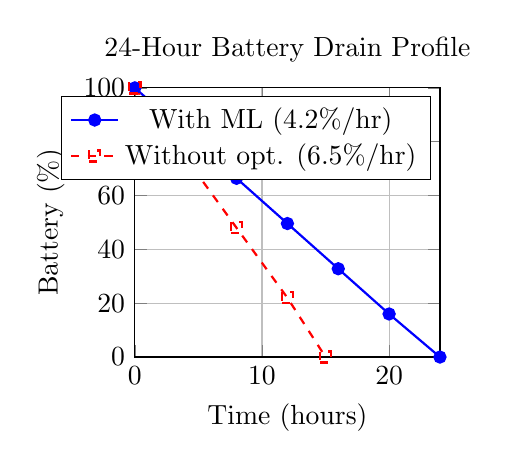
\begin{tikzpicture}
\begin{axis}[
    xlabel={Time (hours)}, ylabel={Battery (\%)},
    xmin=0, xmax=24, ymin=0, ymax=100,
    legend pos=north east, grid=major,
    width=0.45\textwidth, height=5cm,
    title={24-Hour Battery Drain Profile},
]
\addplot[thick, blue, mark=*] coordinates {
    (0,100) (4,83.2) (8,66.4) (12,49.6) (16,32.8) (20,16.0) (24,0)
};
\addlegendentry{With ML (4.2\%/hr)}
\addplot[thick, red, dashed, mark=square] coordinates {
    (0,100) (4,74) (8,48) (12,22) (15,0)
};
\addlegendentry{Without opt. (6.5\%/hr)}
\end{axis}
\end{tikzpicture}
\caption{Battery drain comparison with and without optimization.}
\label{fig:battery}
\end{figure}

\subsection{Edge vs. Cloud Accuracy}

\begin{table}[H]
\centering
\caption{Edge vs. Cloud Accuracy}
\label{tab:edge_cloud}
\begin{tabular}{lccc}
\toprule
\textbf{Task} & \textbf{Edge TFLite} & \textbf{Cloud} & \textbf{Gap} \\
\midrule
Activity Classification & 34.3\% & 85.8\% (XGBoost) & 51.5\% \\
Anomaly Detection (F1) & -- & 0.995 (GradBoost) & -- \\
Heuristic Fallback & $\sim$75\% & -- & -- \\
\bottomrule
\end{tabular}
\end{table}

Edge models serve as a privacy-preserving first pass; cloud inference provides the definitive score with human-readable anomaly reasons.
